\ylDisplay{Lasketiir} % Ülesande nimi
{Aigar Vaigu} % Autor
{piirkonnavoor} % Voor
{2016} % Aasta
{G 6} % Ülesande nr.
{4} % Raskustase
{
% Teema: Dünaamika
\ifStatement
Siselasketiirus tulistatakse vintpüssist, mille kuuli kiirus $v=\SI{320}{m/s}$, kaugusel $s=\SI{30}{m}$ olevat märklauda. Laskur sihib püssiga samal kõrgusel olevat märki ja tabab seda otse kümnesse. Hinnake, kui kaugele sihtmärgist satuks kuul, kui relva enne laskmist keerata ümber sihtimistelje 180 kraadi? Õhutakistusega mitte arvestada.
\fi


\ifHint
Kuul liigub mööda paraboolselt trajektoori, kusjuures kiiruse horisontaalne komponent püsib konstantne, st $v_x = \const = v\cos\alpha$, ning vertikaalne komponent on ühtlaselt kiirenev $v_y = v\sin\alpha - gt$.
\fi


\ifSolution
Vastavalt ülesande tekstile ei arvesta me õhutakistust.
Esmalt tuleb leida, missuguse nurga $\alpha$ all on relva vintraud suunatud ülespoole, et tabada märklaua keskmesse ehk \enquote{kümnesse} vintpüssi normaalse asendi korral. Kuuli trajektoor on sümmeetriline, seega kuuli kogu lennuaeg $t$ on kaks korda suurem kui aeg $t\idx{tipp}$, mis kulub trajektoori kõrgeimasse punkti jõudmiseks (vt joonis).
\begin{figure}[h!]
	\centering
	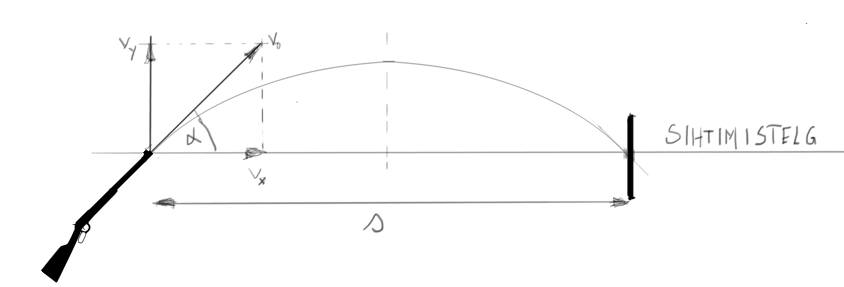
\includegraphics[scale=0.55]{2016-v2g-06-Lasketiir-1.PNG}
	%\caption{Joonis 1}
	%\label{fig:lasketiir_1}
\end{figure}

Järgnevalt kirjeldame kuuli liikumist liikumisvõrranditega horisontaalse liikumise jaoks
$$
s=v_{x}t
$$
ja vertikaalse liikumise jaoks
$$
v_{y}-gt\idx{tipp}=v_{y}-g\frac{t}{2}=0,
$$
kus $g$ on raskuskiirendus \SI{9,81}{m/s^2}, $s$ märklaua kaugus \SI{30}{m} ning $v_x$ ja $v_y$ vastavalt horisontaal- ja verikaalsuunaline algkiirus.

Neid kahte võrrandit kombineerides saame leida nurga $\alpha$:
\begin{align*}
s=v_{x}t & \Rightarrow t=\frac{s}{v_{x}},\\
v_{y}-g\frac{t}{2} & = 0,\\
v_{y}-g\frac{s}{2v_{x}} & = 0,\\
2v_{x}v_{y} & = gs.
\end{align*}
Avaldame viimses reas $v_x$ ja $v_y$ algkiiruse $v_o$ ja trigonomeetriliste funktsioonide kaudu ning kasutame kahekordse nurga siinuse valemit 
$\sin2\alpha = 2\sin\alpha\cos\alpha$. Saame, et 
\begin{align*}
2v_{x}v_{y} & = gs,\\
2v_{0}^{2}\sin\alpha\cos\alpha & = gs,\\
v_{0}^{2}\sin2\alpha & = gs,\\
\sin2\alpha & = \frac{gs}{v_{0}^{2}}.
\end{align*}

\begingroup
\setlength{\columnsep}{1pt}
\begin{wrapfigure}[15]{r}{0.35\textwidth}
	\vspace{-20pt}
	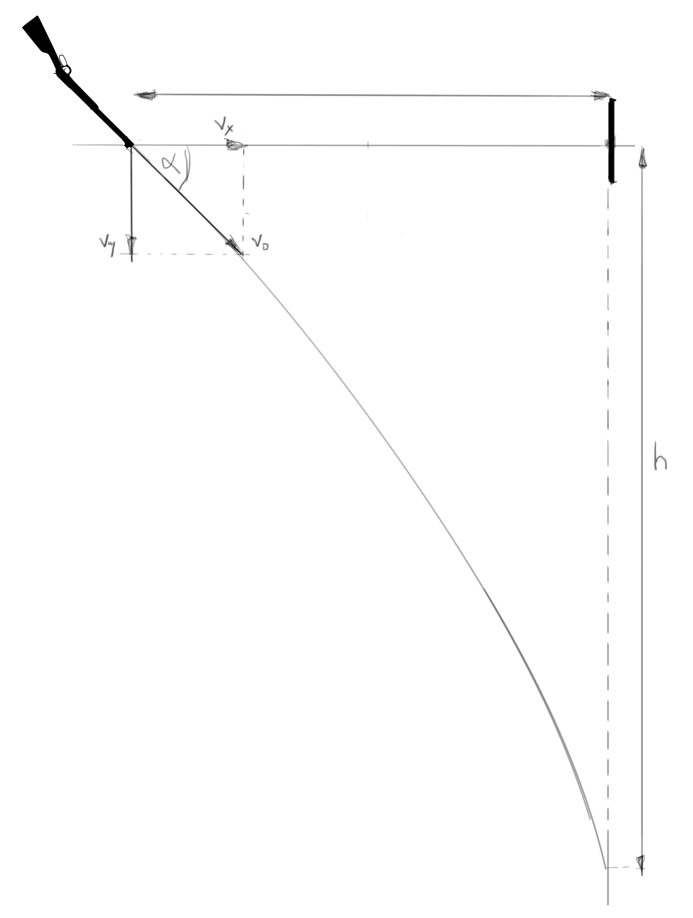
\includegraphics[width = \linewidth]{2016-v2g-06-Lasketiir-2.PNG}
	%\caption{Joonis 2}
	%\label{fig:lasketiir_1}
\end{wrapfigure}
Kui nüüd keerata relva ümber sihtimistelje $180$ kraadi, siis kui enne oli relvatoru nurga $\alpha$ võrra suunatud üles, on relvatoru nüüd sama nurga jagu suunatud alla (vt joonis), seega jäävad kuuli horisontaal- ja vertikaalsuunalised kiirused oma arvväärtuselt samaks.

Kuuli märklaua tabamise koha leiame kuuli vertikaalsuunalisest liikumisvõrrandist, arvestades et kuuli lastakse allapoole:
$$
h=v_{y}t+\frac{gt^2}{2}.
$$
Asendame liikumisvõrrandisse kuuli lennuaja $t$ ja vertikaalsuunalise kiiruse $v_y$ horisontaalsuunalise kiiruse $v_x$ kaudu vastavalt $t=s / v_x$ ja $v_y = gs/2v_x$. Saame:
\begin{align*}
h & = v_{y}\frac{s}{v_{x}}+\frac{gs^2}{2v_{x}^2},\\
h & = \frac{gs}{2v_x}\frac{s}{v_{x}}+\frac{g}{2}\Big(\frac{s}{v_{x}}\Big)^2,\\
h & = \frac{gs^2}{v_{x}^2},\\
h & = \frac{gs^2}{v_{0}^2\cos^2\alpha}.
\end{align*}
\endgroup

Kuna nurk $\alpha$ on meil teada, saame arvutada koha, kus kuul märklauda tabab.

Võib aga kasutada trigonomeetria seoseid. Saame:
\begin{align*}
h & = {gs^2 \over v_{0}^2\cos^2\alpha}\\
& = {gs^2 \over v_{0}^2}{2 \over 1+\cos2\alpha}\\
& = {gs^2 \over v_{0}^2}{2 \over 1+\sqrt{1-\sin^2 2\alpha}}\\
& = {gs^2 \over v_{0}^2}{2 \over 1+\sqrt{1-\Big({gs \over v_0^2}\Big)^2}}\\
& = {2gs^2 \over v_0^2+\sqrt{v_0^4-(gs)^2}}.
\end{align*}
Rehkendus annab tulemuseks:
$$
h  = \frac{2\cdot \SI{9,81}{m/s^2} \cdot (\SI{30}{m})^2}{(\SI{320}{m/s})^2+\sqrt{(\SI{320}{m/s})^4-(\SI{9,81}{m/s^2} \cdot \SI{30}{m})^2}} \approx \SI{8,6}{cm}.
$$
\fi


\ifEngStatement
% Problem name: Shooting range
In an indoors shooting range a target is shot at with a rifle, the speed of the rifle’s bullet is $v=\SI{320}{m/s}$ and the target is at a distance $s=\SI{30}{m}$. The shooter is aiming the rifle at the target which is at the same height as the rifle and shoots the target exactly in the middle. Evaluate how far from the target would the bullet land if the rifle is turned 180 degrees around the aiming axis. Do not account for air resistance.
\fi


\ifEngHint
The ball is moving along a parabolic trajectory, moreover the horizontal component of the velocity stays constant, meaning $v_x = \const = v\cos\alpha$ and the vertical component is evenly accelerating $v_y = v\sin\alpha - gt$.
\fi


\ifEngSolution
\begin{figure}[h!]
	\centering
	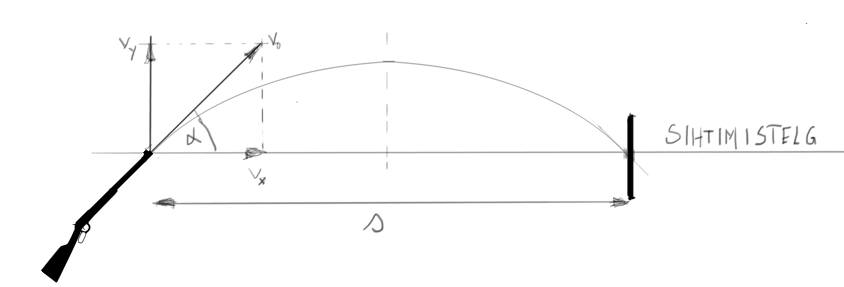
\includegraphics[scale=0.55]{2016-v2g-06-Lasketiir-1.PNG}
	%\caption{Joonis 1}
	%\label{fig:lasketiir_1}
\end{figure}
According to the problem’s text we neglect air resistance. First we have to find at what angle $\alpha$ is the rifle barrel directed upwards to hit the target into the center. The trajectory of the bullet is symmetrical, thus the total flight time of the bullet $t$ is two times bigger than the time $t\idx{tip}$ that it takes to reach the highest point of the trajectory (see figure).\\
Next we describe the horizontal motion of the bullet with equations of motion
$$
s=v_{x}t
$$ 
and the vertical motion
$$
v_{y}-gt\idx{tip}=v_{y}-g\frac{t}{2}=0,
$$ 
where $g$ is the gravitational acceleration $\SI{9,81}{m/s^2}$, $s$ the distance of the target (30 m) and $v_x$ and $v_y$ respectively horizontal and vertical initial speed.\\
Combining these two equations we can find the angle $\alpha$:
\begin{align*}
s=v_{x}t & \Rightarrow t=\frac{s}{v_{x}},\\
v_{y}-g\frac{t}{2} & = 0,\\
v_{y}-g\frac{s}{2v_{x}} & = 0,\\
2v_{x}v_{y} & = gs.
\end{align*}
Let us express $v_x$ and $v_y$ from the last line with the help of initial speed $v_o$ and trigonometric functions and use the double-angle formula of sine $\sin2\alpha = 2\sin\alpha\cos\alpha$. We get that
\begin{align*}
2v_{x}v_{y} & = gs,\\
2v_{0}^{2}\sin\alpha\cos\alpha & = gs,\\
v_{0}^{2}\sin2\alpha & = gs,\\
\sin2\alpha & = \frac{gs}{v_{0}^{2}}.
\end{align*} 
\begin{wrapfigure}[15]{r}{0.35\textwidth}
	\vspace{-20pt}
	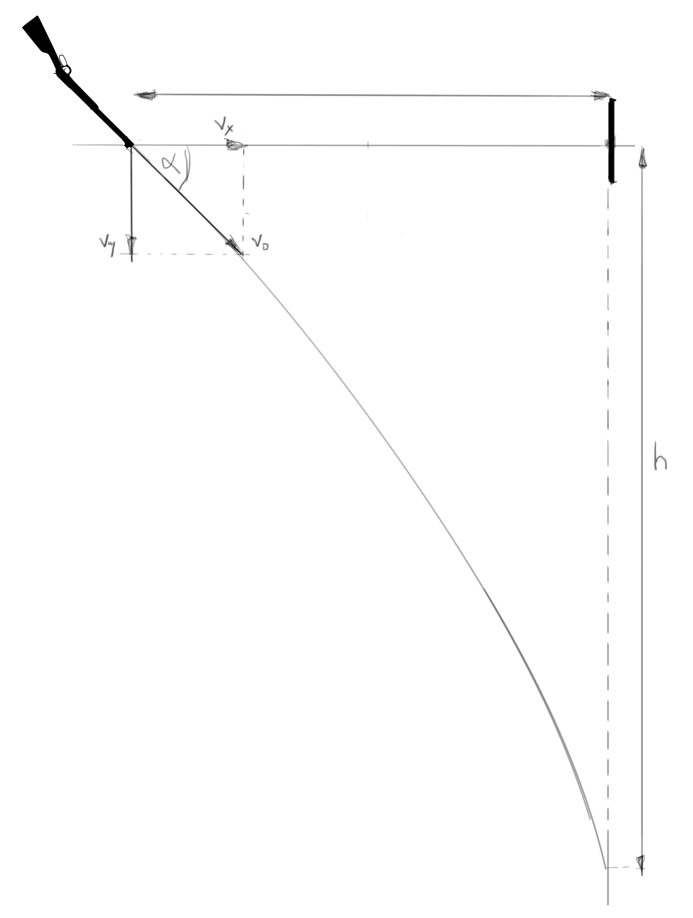
\includegraphics[width = \linewidth]{2016-v2g-06-Lasketiir-2.PNG}
	%\caption{Joonis 2}
	%\label{fig:lasketiir_1}
\end{wrapfigure}
If the rifle would now be turned $180$ degrees around the aiming axis, the barrel is directed downwards at the angle $\alpha$ (see figure) as opposed to it previously being directed upwards at the same angle. Thus, the numerical values of the bullet’s horizontal and vertical velocities stay the same. From the bullet’s vertical directed equation of motion we find the location where the bullet hits the target, while considering that the bullet is shot downwards:
$$
h=v_{y}t+\frac{gt^2}{2}.
$$ 
Let us replace the time $t$ of the bullet’s flight into the equation of motion and the vertical velocity $v_y$ from the horizontal velocity $v_x$ respectively $t=s / v_x$ and $v_y = gs/2v_x$. We get:
\begin{align*}
h & = v_{y}\frac{s}{v_{x}}+\frac{gs^2}{2v_{x}^2},\\
h & = \frac{gs}{2v_x}\frac{s}{v_{x}}+\frac{g}{2}\Big(\frac{s}{v_{x}}\Big)^2,\\
h & = \frac{gs^2}{v_{x}^2},\\
h & = \frac{gs^2}{v_{0}^2\cos^2\alpha}.
\end{align*} 
Because we know the angle $\alpha$ we can find the location where the bullet hits the target. We can use trigonometric formulas. We get:
\begin{align*}
h & = {gs^2 \over v_{0}^2\cos^2\alpha}\\
& = {gs^2 \over v_{0}^2}{2 \over 1+\cos2\alpha}\\
& = {gs^2 \over v_{0}^2}{2 \over 1+\sqrt{1-\sin^2 2\alpha}}\\
& = {gs^2 \over v_{0}^2}{2 \over 1+\sqrt{1-\Big({gs \over v_0^2}\Big)^2}}\\
& = {2gs^2 \over v_0^2+\sqrt{v_0^4-(gs)^2}}.
\end{align*}
From where:
$$
h  = \frac{2\cdot \SI{9,81}{m/s^2} \cdot (\SI{30}{m})^2}{(\SI{320}{m/s})^2+\sqrt{(\SI{320}{m/s})^4-(\SI{9,81}{m/s^2} \cdot \SI{30}{m})^2}} \approx \SI{8,6}{cm}.
$$
\fi
}